\documentclass[a4paper]{article} 

%utf8 or latin1 ?
\usepackage[utf8]{inputenc}
\usepackage[T1]{fontenc}
\usepackage[frenchb]{babel}
\usepackage{graphicx}
\usepackage{float}
\usepackage{soul}

\graphicspath{{images/}{Maquettes/PNG/}{UML/}}
\title{Rapport de conception}
\author{Adonis \bsc{Najimi},\\
 Valentin \bsc{Stern},\\
 Vincent \bsc{Albert},\\
 Théo \bsc{Gerriet}}
\date{\today}

\begin{document}

\maketitle
\newpage

\section{Présentation du projet}
	\subsection{Cahier des charges fonctionnel}
		Priorité haute\newline
- Analyse et enregistrement des notes\newline
- Envoi des partitions\newline
- Accordeur\newline
- Jouer une partition\newline
\newline
Priorité moyenne\newline
- Apprentissage de la composition\newline
\newline
Priorité basse\newline
- Analyse automatique d'une partition\newline

\section{Client C++}
	\subsection{Présentation du client}
		La fonctionnalité majeure du client et de permettre à l'utilisateur de composer et enregistrer ses propres musiques en jouant avec sa guitare. Il n'aura qu'a jouer ce qu'il veut et l'application traitera les notes jouées et les enregistrera dans une partition. Il pourra par la suite modifier les notes de la partition en cas d'erreur. 

Le client comporte d'autres fonctionnalitées annexes non essentielles mais intéressantes cependant.
L'utilisateur pourra, avant de commencer à jouer, accorder sa guitare afin de jouer le plus juste possible.
Le client a pour but de permettre à l'utilisateur de composer ses chansons, et il y aura donc une partie permettant l'apprentissage des bases de la composition à la guitare de manière interactive. Il pourra apprendre à créer des accords, jouer sur différentes gammes ou encore apprendre le rythme.

Une fonctionnalitée permettant d'envoyer directement sa partition au serveur web sera également présente afin de simplifier le partage de ses créations.
	\subsection{Description du contenu du modele}
		Cette partie de l'application est principalement basée sur l'analyse et l'enregistrement des notes jouées par 
l'utilisateur. Le principe est d'analyser en temps réel les fréquences à la base du son de la guitare, et de faire en sort de constituer un accord
avec les notes ayant le volume le plus fort et l'enregistrer. De plus, le modèle comporte également toutes les informations sur les préférences
de l'utilisateur pour l'application,   ainsi que des fonctions pour enregistrer les données. Nous avons choisi de sauvegarder les fichiers au format JSON.\newline

\begin{figure}[H]
\centering
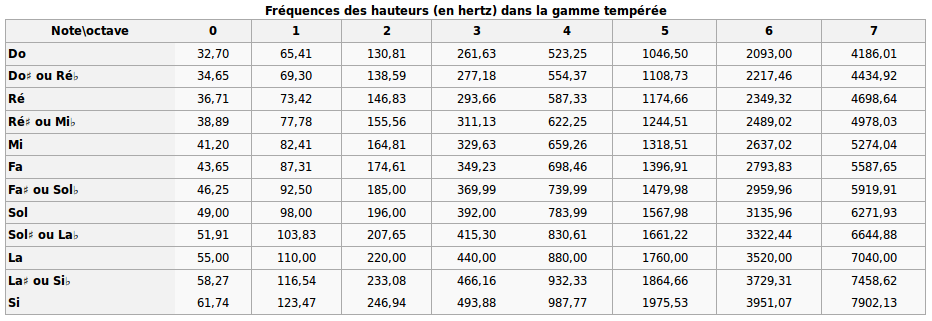
\includegraphics[scale=0.5]{Frequences}
\caption{Toutes les frequences possibles}
\end{figure}
	\subsection{UML du modele de l'application}
		\begin{figure}[H]
\centering
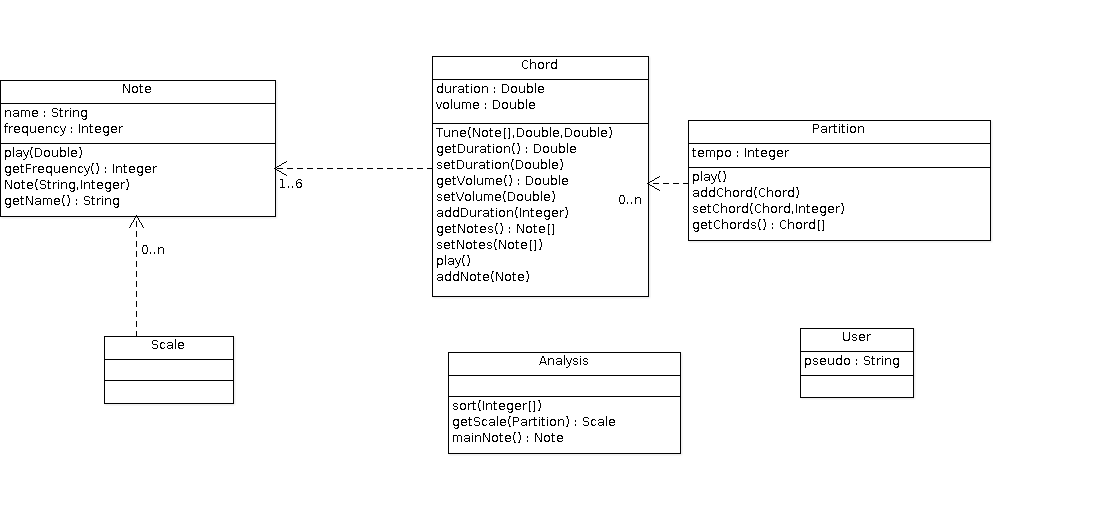
\includegraphics[scale=0.4]{ModelUML}
\caption{UML du modele}
\end{figure}

La classe Note représente une Note qui n'est pas jouée, c'est-à-dire qu'elle contient la définition d'une note seulement.\newline
La classe Chord permet donc de représenter de 1 à 6 note jouée simultanément tel un accord à la guitare.\newline
La classe Partition représente donc une partition comme l'utilisateur va la voir.\newline
La classe Analysis propose différentes fonctions essentielles à l'application. Cette classe propose également des fonctionnalités pour l'apprentissage de la composition de musiques.\newline
La classe Scale représente une gamme. Une gamme est une suite de notes, et la classe est donc composée d'un certain nombre de note.
La classe User est présente pour enregistrer le pseudonyme de l'utilisateur pour pouvoir envoyer des partitions sur le site.
Lorsque l'utilisateur va jouer une note, le logiciel va récupérer toutes les fréquences entrant par le micro et les trier en fonction de leur volume. Il est donc aisé par la suite de trouver quelles sont les notes qui sont le plus jouées.

	\subsection{Algorithmes}
		% \begin{tabbing}

% \ul{fonction} analyser(frequences : \ul{tableau entier}[0..n], n : \ul{entier}, seuilMin : \ul{entier}) : \ul{tableau Accord}\\
% \ul{debut}\\
% frequences <- trier(frequences)\\
% i <- 0\\
% complet <- faux\\
% \ul{Tant que} i < n \ul{et} \ul{non} complet \ul{faire}\\
%     freq <- frequences[i]\\
%     \ul{Si} freq > seuilMin \ul{et} \ul{non} present(retour, freq)\\
%     \ul{alors}\\
%         ajouter(retour, freq)\\
%         \ul{Si} taille(retour) > 5\\
%         \ul{alors}\\
%             complet <- vrai\\
%         \ul{fsi}\\
%     \ul{fsi}\\
% \ul{ftantque}\\
% \ul{retourne} retour\\
% \ul{fin}\\
% \end{tabbing}
% \newline
% \ul{lexique}\newline

\ul{Structures de donnees utilisees dans les algorithmes:}\newline
\ul{Note} < frequence : \ul{entier}, nom : \ul{chaine} >\newline
\ul{EntreeMicro} : Type correspondant à l'entrée micro de l'ordinateur. Il permet de récupérer les fréquences à un certain instant\newline
% Algo de récupérer une note avec sa fréquence
Récupérer une note grâce à sa fréquence\newline
\begin{tabbing}
\kill XX\=XX\=XX\=XX\=XX\=XX\=XX\=XX\=XX\=XX\=
\kill
\ul{fonction} recupererNote(frequence : \ul{entier}, notes : \ul{Note[0..n]}, n : \ul{entier}) : Note\\
\ul{debut}\\
\>min <- 0\\
\>max <- n\\
\>trouve <- faux\\
\>\ul{Tant que} min <= max \ul{et} \ul{non} trouve \ul{faire}\\
    \>\>indice <- (max + min) /2 \\
    \>\>frequenceNote <- notes[indice].frequence\\
    \>\>\ul{Si} frequence = frequenceNote\\
    \>\>\ul{alors}\\
        \>\>\>retour <- notes[indice]\\
        \>\>\>trouve <- vrai\\
    \>\>\ul{sinon}\\
        \>\>\>\ul{Si} frequence < frequenceNote\\
        \>\>\>\ul{alors}\\
            \>\>\>\>max <- indice\\
        \>\>\>\ul{sinon}\\
            \>\>\>\>min <- indice\\
        \>\>\>\ul{fsi}\\
    \>\>\ul{fsi}\\
\>\ul{ftantque}\\
\>\ul{Si} \ul{non} trouve\\
\>\ul{alors}\\
    \>\>retour <- notes[min]\\
\>\ul{fsi}\\
\>\ul{retourne} retour\\
\ul{fin}\\
\end{tabbing}
\ul{lexique}\newline
frequence : \ul{entier} : Fréquences de la note à récupérer\newline
notes : \ul{Note[0..n]} : Toutes les notes possibles\newline
n :  \ul{entier} : Nombre de notes possibles\newline
max : \ul{entier} : indice maximal dans le tableau\newline
min : \ul{entier} : indice minimal dans le tableau\newline
trouve : \ul{booleen} : Booléen à vrai si on a trouvé la note (avec exactement la même fréquence)\newline
indice : \ul{entier} : Indice en cours dans le tableau\newline
frequenceNote : \ul{entier} : Frequence de la note en cours d'analyse\newline
retour : \ul{Note} : Note correspondant à la fréquence\newline

Fonction de placement nécessaire à la fonction trier\newline

\begin{tabbing}
\kill XX\=XX\=XX\=XX\=XX\=XX\=XX\=XX\=XX\=XX\=
\kill
\ul{fonction} placer(tab : \ul{InOut} \ul{tableau entier}[0..n], n : \ul{entier}, inf : \ul{entier}, sup : \ul{entier}) : \ul{entier}\\
\ul{debut}\\
    \>inda <- inf\\
    \>a <- tab[inf]\\
    \>inf <- inf + 1\\
    \>\ul{Tant que } sup >= inf \ul{faire}\\
        \>\>\ul{Si} tab[inf] > a\\
        \>\>\ul{alors}\\
            \>\>\>\ul{Tant que} sup >= inf \ul{ou} tab[sup] > a \ul{faire}\\
                \>\>\>\>sup <- sup - 1\\
            \>\>\>\ul{ftantque}\\
            \>\>\>temp <- tab[sup]\\
            \>\>\>tab[sup] <- tab[inf]\\
            \>\>\>tab[inf] <- temp\\
            \>\>\>sup <- sup - 1\\
        \>\>\ul{fsi}\\
        \>\>inf <- inf + 1\\
    \>\ul{ftantque}\\
    \>temp <- tab[sup]\\
    \>tab[sup] <- tab[inda]\\
    \>tab[inda] <- temp\\
    \>\ul{retourne} sup\\
\ul{fin}\\
\end{tabbing}

Fonction de tri des fréquences\newline
\begin{tabbing}
\kill XX\=XX\=XX\=XX\=XX\=XX\=XX\=XX\=XX\=XX\=
\kill
\ul{fonction} trier(frequences : \ul{tableau entier}[0..n], n : \ul{entier}, inf : \ul{entier}, sup : \ul{entier})\\
\ul{debut}\\
    \>\ul{Si} inf < sup\\
    \>\ul{alors}\\
        \>\>indice <- placer(frequences, inf, sup)\\
        \>\>trier(frequences, n, inf, indice - 1)\\
        \>\>trier(frequences, n, indice + 1, sup)\\
    \>\ul{fsi}\\
\ul{fin}\\ 
\end{tabbing}

Montrer la note principale(pour l'accordeur)\newline
\begin{tabbing}
\kill XX\=XX\=XX\=XX\=XX\=XX\=XX\=XX\=XX\=XX\=
\kill
\ul{fonction} montrerNote(mic : \ul{entreeMicro})\\
\ul{debut}\\
\>accorder <- vrai\\
\>\ul{Tant que}\\
    \>\>freqs <- recupererFrequences(mic)\\
    \>\>freqs <- trier(freqs)\\
    \>\>\ul{ecrire} recupererNote(freqs[0])\\
\>\ul{ftantque}\\
\ul{fin}\\
\end{tabbing}

\ul{lexique}\newline
mic : \ul{entreeMicro} : Entrée micro utilisée\newline
accorder : \ul{booleen} : Booleen à vrai si on continue à accorder. Il peut être changer grâce à un clic dans l'application\newline
freqs : freqs : \ul{tableau entier}[0..n] : Frequences envoyées par mic\newline
\newline

Enregistrement d'une partition\newline
%Enregistrement d'une partition
\begin{tabbing}
\kill XX\=XX\=XX\=XX\=XX\=XX\=XX\=XX\=XX\=XX\=
\kill
\ul{fonction} enregistrer(mic : \ul{entreeMicro}, seuilHaut :  \ul{entier}, seuilBas : \ul{entier}, tempo : \ul{entier}) : \ul{Partition}\\
\ul{debut}\\
\>enregistrer <- vrai\\
\>j <- 0\\
\>\ul{Tant que} enregistrer \ul{faire}\\
    \>\>frequences <- recupererFrequences(mic)\\
    \>\>frequences <- trier(frequences)\\
    \>\>complet <- faux\\
    \>\>fini <- faux\\
    \>\>i <- 0 \\
    \>\>\ul{Tant que} \ul{non} complet \ul{et} \ul{non} fini \ul{faire}\\
        \>\>\>frequence <- frequences[i]\\
        \>\>\>\ul{si} frequence > seuilHaut\\
        \>\>\>\ul{alors}\\
            \>\>\>\>ajouter(freqs, accord)\\
            \>\>\>\>j <- j + 1\\
        \>\>\>\ul{sinon}\\
            \>\>\>\>\ul{si} frequence > seuilBas\\
            \>\>\>\>\ul{alors}\\ 
                \>\>\>\>\>ajouterTemps(retour[j], tempo / 16)\\
            \>\>\>\>\ul{sinon}\\
                \>\>\>\>\>fini <- vrai\\
        \>\>\>\ul{fsi}
    \>\>\ul{ftantque}\\     
    \>\>i <- i + 1\\  
    \>\>attendre(tempo / 16)\\
\>\ul{ftantque}\\
\>\ul{retourne} retour \\
\ul{fin}\\
\end{tabbing}

Nous attendons pendant tempo / 16 car c'est la plus petite unité de temps représentable dans une partition. L'utilisateur doit rentrer le tempo dans lequel il compte jouer.



	\subsection{UML de l'interface graphique}
		\paragraph{}
	L'interface graphique sera codée en C++ et respectera le modèle MVC. \\
	Ainsi seul le contrôleur modifiera le modèle, tandis que la classe NoSkin, représentant l'interface,
	ne fera qu'afficher les données. \\
	Ces deux classes sont donc représentées sur l'UML et sont complémentées par des classes complémentaires
	telles que la classe FormatException qui permet de gérer plus finement la conversion JSON/Objet.\\
	Les classes TabWidget, Options et Chord seront utilisées par NoSkin pour créer les fenêtres de 
	l'accordeur, des paramètres et le widget particulier de la tablature.

\begin{figure}[H]

	\centering 
	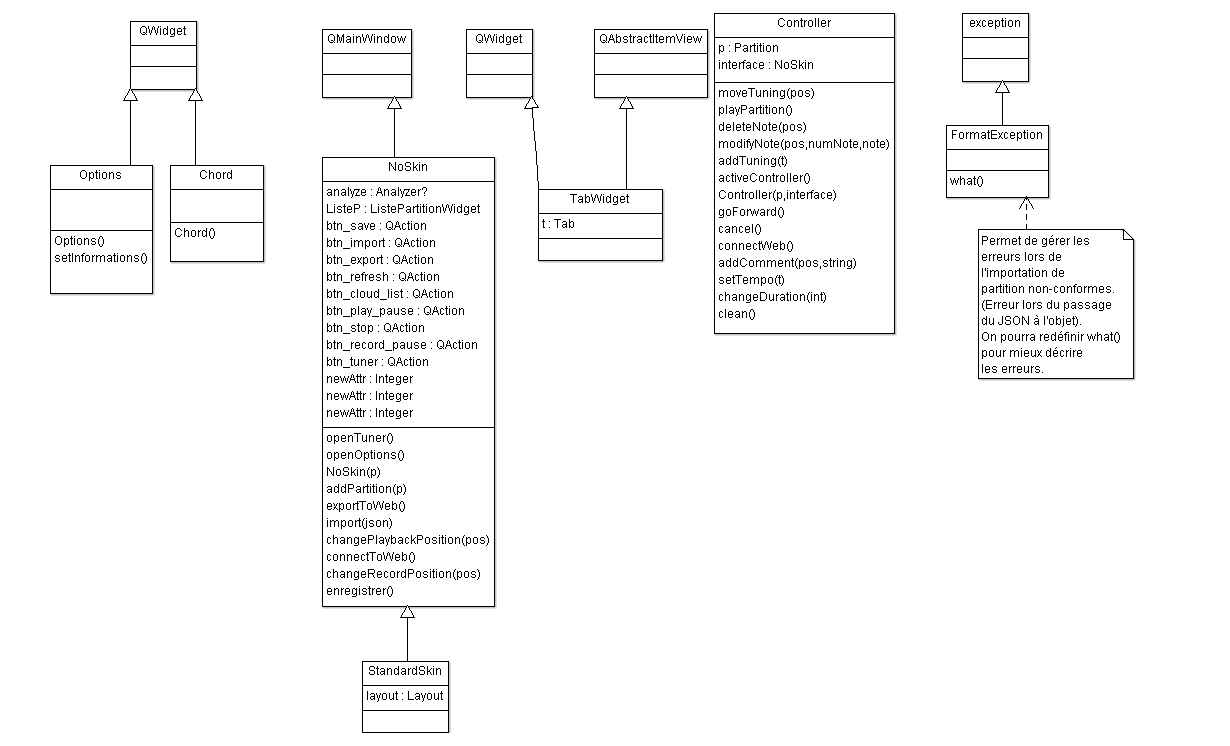
\includegraphics[scale=0.3]{GUI_UML}
		\caption{UML de l'interface graphique}
			

\end{figure}


	\subsection{Maquettes du client}
		
%We begin by creating the main page of the client
\begin{figure}[H]

	\centering 
	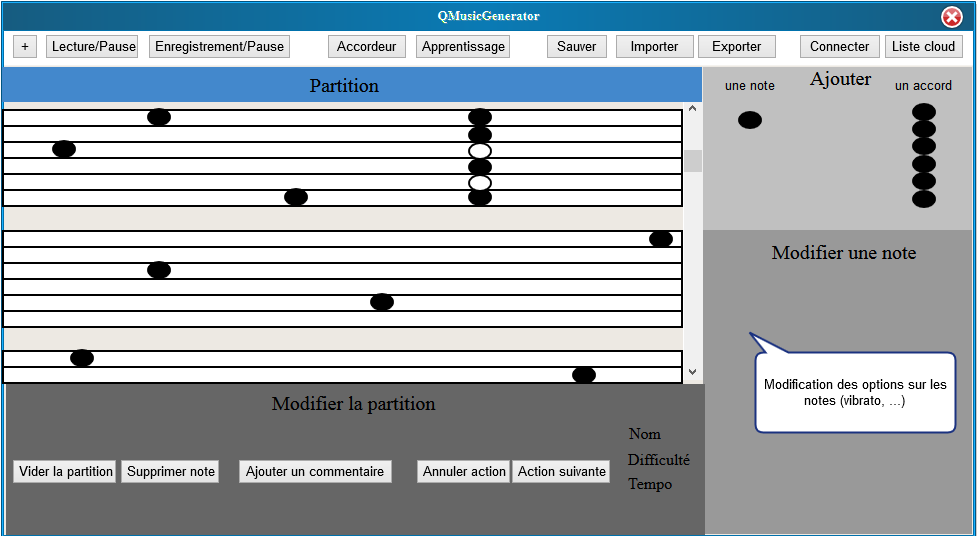
\includegraphics[scale=0.4]{main_page}
		\caption{Page principale du client}
			Cette fenêtre est la fenêtre principale de notre client. A partir de celui-ci, il sera possible
			de créer des partitions vierges, d'en ouvrir des préexistantes, d'en lire et d'enregistrer des 
			notes à partir de l'entrée audio ainsi que de les sauvegarder. \\
			Mais il sera aussi possible d'ouvrir un accordeur, de télécharger des partitions hébergées sur le
			site web, et d'en uploader. \\
			Il sera en effet possible de connecter directement le client avec le site à l'aide des 
			identifiants de l'utilisateur. \\
			De plus, il y aura aussi évidemment toutes les options permettant de modifier la partition en 
			cours, tels que son nom, sa difficulté, son tempo, ... \\
			Enfin, on pourra modifier la partition manuellement en déplaçant les notes ou en en ajoutant. 

\end{figure}

%Then the options list
\begin{figure}[H]

	\centering 
	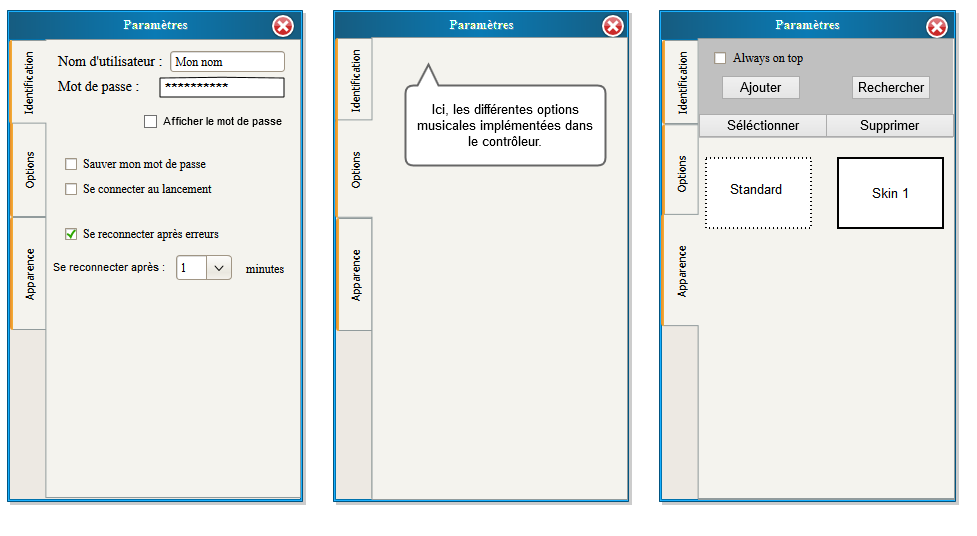
\includegraphics[scale=0.4]{parameters}
		\caption{Fenêtre des paramètres du logiciel}
			Cette fenêtre permettra de modifier les paramètres du logiciel. \\
			Cela recouvre les paramètres d'authentification, ceux spécifiques à la synthèse de musique en
			elle-même, mais aussi l'apparence du client via l'utilisation de skins.

\end{figure}

%And the tablatures list
\begin{figure}[H]

	\centering 
	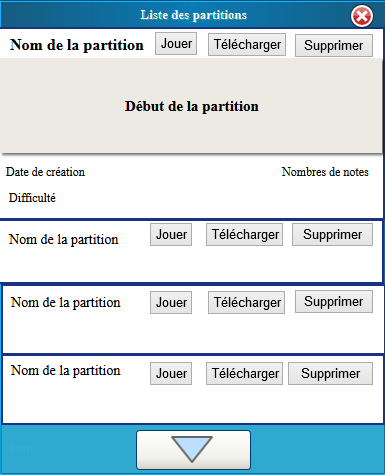
\includegraphics[scale=0.6]{tab_list}
		\caption{Fenêtre des listes de partitions hébergées sur le site web}
			Cette fenêtre listera toutes les partitions que l'utilisateur a uploadé sur le site internet si 
			celui-ci est connecté. \\
			A partir de cette fenêtre, il pourra soit les supprimer du site web, soit les télcharger, ou 
			encore les jouer.
\end{figure}
%Finally, we put the chord
\begin{figure}[H]

	\centering 
	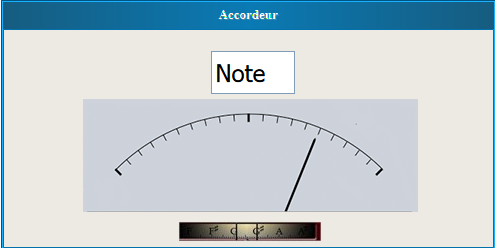
\includegraphics[scale=0.8]{chord}
		\caption{Accordeur}
			Cette fenêtre affichera un accordeur qui analysera l'entrée sonore pour permettre à l'utilisateur
			de réaccorder son instrument directement depuis le logiciel.

\end{figure}

	\subsection{Liaison avec l'application web}
		\paragraph{}
	Afin de communiquer avec l'application web, le client sera doté d'un module réseau qui enverra et 		
	recevra des requêtes http. Les partitions seront envoyées et reçues en format JSON afin de faciliter 
	ces échanges. \\
	Le JSON aura format semblable à ceci :
	
		\begin{tt}
			\{ \\
				“Name” : “string”, \\
				“Tempo” : 0, \\
				“private” : true/false \\
				“tunes” : [\{ \\
					“volume” : 0-1, \\
					“nb\_notes” : 0, \\
					“temps” : “croche”, \\
					“notes” : [\{ \\
						“name” : “do-la-…”, \\
						“frequence” : 0 \\
					\}] \\
				\}]	 \\
			\}
		\end{tt}
\section{Application Web}
	\subsection{Maquettes d'écran}
		Les differentes maquettes du site permettent d'améliorer la vision des besoins de l'application.
Ces visuels ne sont pas définitifs et sont simplement là pour nous aider à mieux structurer l'application et organiser les objectifs nécessaires à la réalisation de celle-ci.
\begin{figure}[H]

\centering
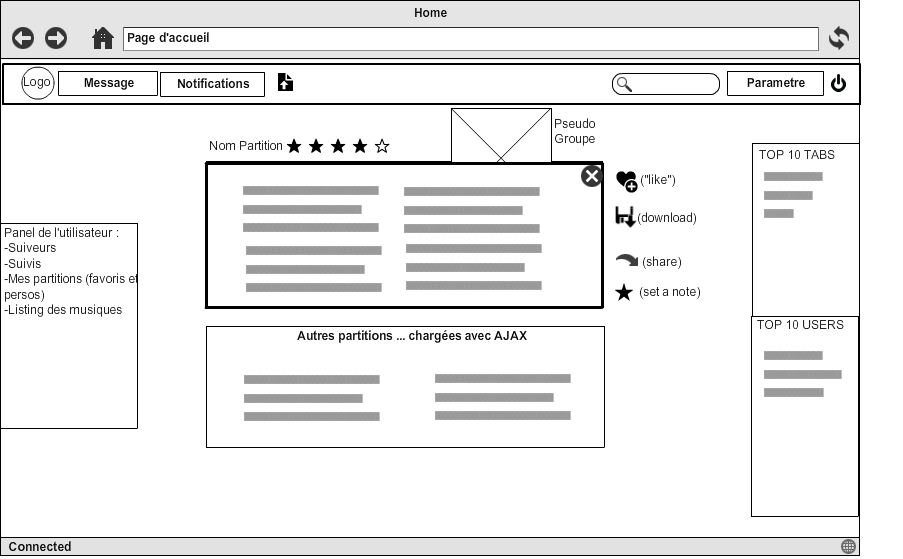
\includegraphics[scale=0.5]{Home}
\caption{Maquette de la page principale du site}
La barre du haut est une barre de menu qui sera
disponible sur toute les pages du site, elle n'est pas
représentée sur toutes les maquettes par soucis de clarté. En
effet, le principal sujet des maquettes suivantes n'est pas
la présence de la barre de menu mais le contenu de celles-ci
\end{figure}

\begin{figure}[H]

\centering
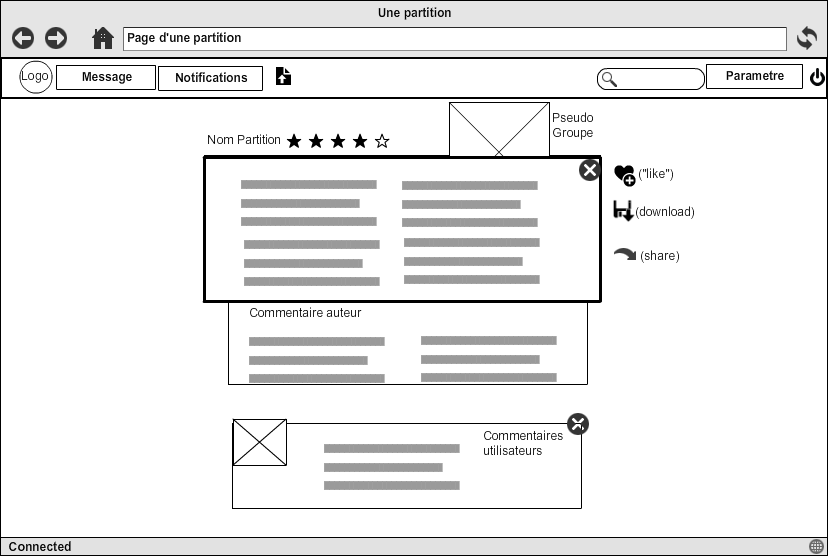
\includegraphics[scale=0.5]{Tab}
\caption{Page principale d'une partition de musique}
\end{figure}


\begin{figure}[H]

\centering
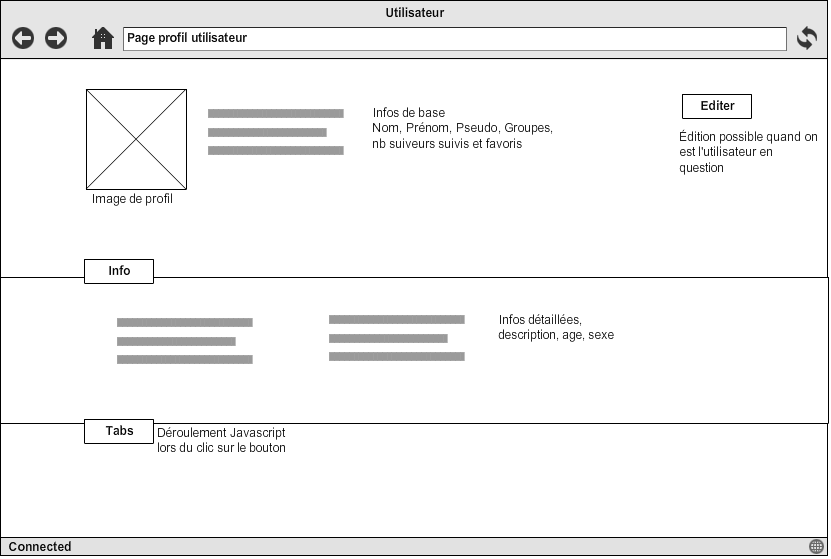
\includegraphics[scale=0.5]{User}
\caption{Page de profil utilisateur}

Cette page permettra à l'utilisateur concerné de modifier ses informations s'il le souhaite.
\newline Les autres utilisateurs verront sur sa page de profil les informations rendues visibles par l'utilisateur en question.
\end{figure}

\begin{figure}[H]

\centering
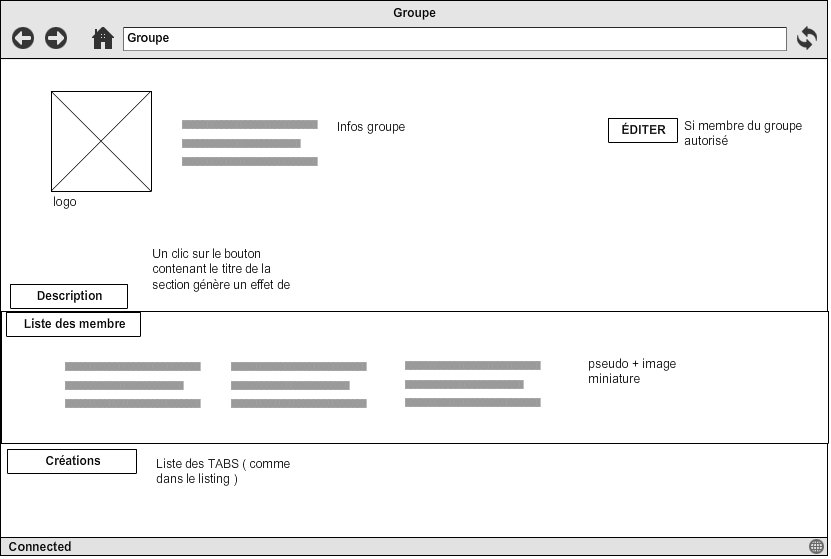
\includegraphics[scale=0.5]{Group}
\caption{Page d'un groupe de musique}

Cette page permettra de modifier le groupe si l'utilisateur en possède les droits.
\newline Cette page contiendra la liste des membres du groupe ainsi que les différentes partitions liées au groupe concerné.
\end{figure}

\begin{figure}[H]
\centering
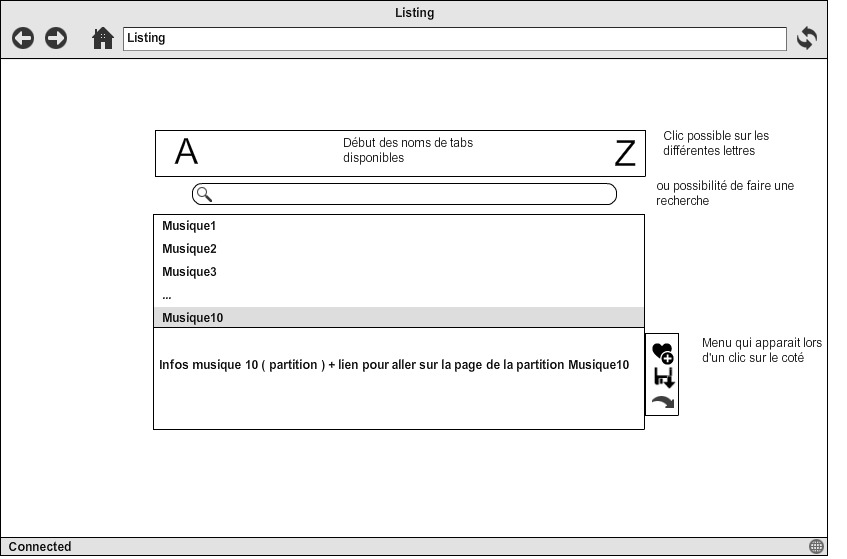
\includegraphics[scale=0.5]{Listing}
\caption{Liste de toutes les partitions}

Le listing des partitions permettra une recherche plus approfondie qu'avec la recherche disponible dans la barre de menu (la barre du haut).

\end{figure}


	\subsection{Modèle Merise MCD}
		\begin{mld}
  \relat{Replies} & (\prim{\foreign{user\_id}}, \prim{\foreign{comment\_id}}, \attr{reply\_date})\\
  \relat{Comments} & (\prim{comment\_id}, \attr{comment\_text}, \foreign{user\_id}, \foreign{tab\_id}, \attr{comment\_date})\\
  \relat{Follows} & (\prim{\foreign{user\_id.1}}, \prim{\foreign{user\_id.2}}, \attr{follow\_date})\\
  \relat{Users} & (\prim{user\_id}, \attr{user\_name}, \attr{user\_birthday}, \attr{user\_nickname}, \attr{user\_description}, \attr{user\_email}, \attr{user\_signup})\\
  \relat{Belongs} & (\prim{\foreign{user\_id}}, \prim{\foreign{group\_id}}, \attr{belong\_date})\\
  \relat{Creates} & (\prim{\foreign{user\_id}}, \prim{\foreign{group\_id}}, \attr{create\_date})\\
  \relat{Tabs} & (\prim{tab\_id}, \attr{tab\_name}, \attr{tab\_file}, \foreign{user\_id}, \attr{tab\_date})\\
  \relat{Likes} & (\prim{\foreign{user\_id}}, \prim{\foreign{tab\_id}})\\
  \relat{Groups} & (\prim{group\_id}, \attr{group\_name}, \attr{group\_creation})\\
  \relat{Makes} & (\prim{\foreign{group\_id}}, \prim{\foreign{tab\_id}}, \attr{make\_date})\\
\end{mld}
	\subsection{Modèle Merise MLD}
		\begin{mld}
  \relat{Replies} & (\prim{\foreign{user\_id}}, \prim{\foreign{comment\_id}}, \attr{reply\_date})\\
  \relat{Comments} & (\prim{comment\_id}, \attr{comment\_text}, \foreign{user\_id}, \foreign{tab\_id}, \attr{comment\_date})\\
  \relat{Follows} & (\prim{\foreign{user\_id.1}}, \prim{\foreign{user\_id.2}}, \attr{follow\_date})\\
  \relat{Users} & (\prim{user\_id}, \attr{user\_name}, \attr{user\_birthday}, \attr{user\_nickname}, \attr{user\_description}, \attr{user\_email}, \attr{user\_signup})\\
  \relat{Belongs} & (\prim{\foreign{user\_id}}, \prim{\foreign{group\_id}}, \attr{belong\_date})\\
  \relat{Creates} & (\prim{\foreign{user\_id}}, \prim{\foreign{group\_id}}, \attr{create\_date})\\
  \relat{Tabs} & (\prim{tab\_id}, \attr{tab\_name}, \attr{tab\_file}, \foreign{user\_id}, \attr{tab\_date})\\
  \relat{Likes} & (\prim{\foreign{user\_id}}, \prim{\foreign{tab\_id}})\\
  \relat{Groups} & (\prim{group\_id}, \attr{group\_name}, \attr{group\_creation})\\
  \relat{Makes} & (\prim{\foreign{group\_id}}, \prim{\foreign{tab\_id}}, \attr{make\_date})\\
\end{mld}
	\subsection{Structure de l'application}
		\paragraph{}
La structure du site suivra le modèle MVC.\\
Des tests unitaires seront utilisés pour s'assurer du bon fonctionnement de l'application.\\
Le site sera à l'aide d'un framework MVC Javascript (Express) pour gérer la partie Serveur et un autre framework complémentaire qui sera utilisé pour les vues et les controllers en particulier (AngularJS).\\
Utiliser Javascript pour coder toute l'application web aussi bien du côté client que du côté serveur nous permettra d'avoir une première approche avec cette technologie qui devient de plus en plus demandée aujourd'hui. Ce qui rend donc ce projet très enrichissant pour notre avenir professionel.
\\
\\
Le site sera donc divisé en trois principales parties : \\
-Views \\
-Controllers \\ 
-Models \\
Plus une partie qui contiendra les routes (ie les chemins d'accès aux différents controllers)
\\

Views : \\ 
-home => représentera l'accueuil du site
-compte => Profil utilisateur \\
-groupe => Profil du groupe \\
-listing => Listing des différents partitions avec option de recherche\\
-topbar => barre du haut qui sera incluse sur toutes les pages\\
-tabpage => page principale d'une partition\\

Controllers: \\
Les controllers seront utilisés pour faire le lien entre le modèle et les différentes vues. De plus ils permettront de gérer les fonctionnalités spécifiques au site. \\
-home.js => controller général \\
-profil.js => controller du compte qui gère le profil utilisateur\\
-groupe.js => controller qui gère les groupes utilisateurs \\
-listing.js => controller qui gère la liste des partitions ainsi que la fonction recherche dans celles-ci\\
-topbare.js => permet de gérer la barre de menu présente sur le haut du site\\
-partition.js  => permet de gérer les fonctionnalités d'une partition en particulier\\
-partition-page.js => controller qui gère la page d'une partition\\

Les modèles suivent l'architecture Active Record. \\
Ils seront donc liés à la base de données (cf MCD et MLD). \\
Une table équivaut donc à un module JavaScript. \\
Ces modules contiendront toutes les méthodes nécessaires au traitement et à la modification du modèle (findById,insert,delete,update ...) et suivront donc l'approche vue en cours. \\
\\

Routes: \\
Chaque lien est une route qui peut contenir une action et qui actionne une méthode du controller lié à la route. \\
Une route est donc un chemin représenté par un URL. \\
Ces routes sont donc le coeur du fonctionnement de l'application Web.\\



\newpage
\tableofcontents


\end{document}